\documentclass{article}

\usepackage[nonatbib]{nips_2018}
\usepackage[numbers,sort&compress]{natbib}

\usepackage[utf8]{inputenc} % allow utf-8 input
\usepackage[T1]{fontenc}    % use 8-bit T1 fonts
\usepackage{hyperref}       % hyperlinks
\usepackage{url}            % simple URL typesetting
\usepackage{booktabs}       % professional-quality tables
\usepackage{amsfonts}       % blackboard math symbols
\usepackage{nicefrac}       % compact symbols for 1/2, etc.
\usepackage{microtype}      % microtypography
\usepackage{amsmath, amssymb, amsthm}
\usepackage{latexsym, caption, subcaption, verbatim}
\usepackage{graphicx, bm, algorithm, algpseudocode}

\newcommand{\btheta}{\ensuremath{\bm{\theta}}}
\newcommand{\opdiag}{\ensuremath{\operatorname{diag}}}
\newcommand{\bx}{\ensuremath{\mathbf{x}}}
\newcommand{\by}{\ensuremath{\mathbf{y}}}
\newcommand{\bt}{\ensuremath{\mathbf{t}}}
\newcommand{\bz}{\ensuremath{\mathbf{z}}}

\title{Learning Stochastic Dynamical Systems via Bridge Sampling}
\author{
 Harish~S. Bhat\\
 Applied Mathematics Unit\\
 University of California, Merced\\
 Merced, CA 95343\\
 \texttt{hbhat@ucmerced.edu} \\
 \And
 Shagun Rawat\\
 Applied Mathematics Unit\\
 University of California, Merced\\
 Merced, CA 95343\\
 \texttt{srawat2@ucmerced.edu}
}

\begin{document}
\maketitle


\begin{abstract}
  We develop algorithms to automate discovery of stochastic dynamical system
  models from noisy, vector-valued time series.  By discovery, we mean 
  learning both a nonlinear drift vector field and a diagonal diffusion matrix 
  for an It\^{o} stochastic differential equation in $\mathbb{R}^d$.  We 
  parameterize the vector field using tensor products of Hermite polynomials,
  enabling the model to capture highly nonlinear and/or coupled dynamics.
  We solve the resulting estimation problem using expectation maximization (EM).
  This involves two steps.  We augment the data via diffusion bridge
  sampling, with the goal of producing time series observed at a higher
  frequency than the original data.  With this augmented data,
  the resulting expected log likelihood maximization problem
  reduces to a least squares problem.  Through experiments on systems with 
  dimensions one through eight, we show that this EM approach enables 
  accurate estimation for multiple time series with possibly irregular 
  observation times.  We study how the EM method performs as a function of
  the noise level in the data, the volume of data, and the amount of data
  augmentation performed.  
\end{abstract}

\section{Introduction}
Traditional mathematical modeling in the sciences and engineering often has as its goal the development of equations of motion that describe observed phenomena.  Classically, these equations of motion usually took the form of deterministic systems of ordinary or partial differential equations (ODE or PDE, respectively).  Especially in systems of contemporary interest in biology and finance where intrinsic noise must be modeled, we find stochastic differential equations (SDE) used instead of deterministic ones.  Still, these models are often built from first principles, after which the model's predictions (obtained, for instance, by numerical simulation) are compared against observed data.

Recent years have seen a surge of interest in using data to automate discovery of ODE, PDE, and SDE models.  These machine learning approaches complement traditional modeling efforts, using available data to constrain the space of plausible models, and shortening the feedback loop linking model development to prediction and comparison to real observations.  We posit two additional reasons to develop algorithms to learn SDE models.  First, SDE models---including the models considered here---have the capacity to model highly nonlinear, coupled stochastic systems, including systems whose equilibria are non-Gaussian and/or multimodal.  Second, SDE models often allow for interpretability.  Especially if the terms on the right-hand side of the SDE are expressed in terms of commonly used functions (such as polynomials), we can obtain a qualitative understanding of how the system's variables influence, regulate, and/or mediate one other. 

In this paper, we develop an algorithm to learn SDE models from high-dimensional time series.  To our knowledge, this is the most general expectation maximization (EM) approach to learning an SDE with multidimensional drift vector field and diagonal diffusion matrix.  Prior EM approaches were restricted to one-dimensional SDE \cite{ghahramani_learning_1999}, or used a Gaussian process approximation, linear drift approximation, and approximate maximization \cite{ruttor_approximate_2013}.  To develop our method, we use diffusion bridge sampling as in \cite{van_der_meulen_reversible_2014, meulen_adaptive_2017}, which focused on Bayesian nonparametric methods for SDE in $\mathbb{R}^1$.  After augmenting the data using bridge sampling, we are left with a least-squares problem, generalizing the work of \cite{brunton_discovering_2016} from the ODE to the SDE context.

In the literature, variational Bayesian methods are the only other SDE learning methods that have been tested on high-dimensional problems \cite{vrettas_variational_2015}.  These methods use approximations consisting of linear SDE with time-varying coefficients \cite{archambeau_variational_2008}, kernel density estimates \cite{batz_variational_2016}, or Gaussian processes \cite{batz_approximate_2017}.  In contrast, we parameterize the drift vector field using tensor products of Hermite polynomials; as mentioned above, the resulting SDE has much higher capacity than linear and/or Gaussian process models.

Many other techniques explored in the statistical literature focus on scalar SDE \cite{nicolau_nonparametric_2007, muller_empirical_2010, verzelen_inferring_2012, bhat_nonparametric_2016}.

As mentioned, differential equation discovery problems have attracted considerable recent interest.  A variety of methods have been developed to learn ODE \cite{brunton_discovering_2016, schon_probabilistic_2017, chen_network_2017, tran_exact_2017, schaeffer_extracting_2017, schaeffer_learning_2017, quade_sparse_2018} as well as PDE \cite{schaeffer_sparse_2013, raissi_machine_2017, rudy_data-driven_2017, raissi_hidden_2018}.  Unlike many of these works, we do not focus on model selection and/or regularization; if needed, our methods can be combined with model selection procedures developed in the ODE context \cite{mangan_inferring_2016, mangan_model_2017}.

\begin{itemize}
\item results 1D, 2D, 3D damped duffing, 3D lorenz
\item plots error of theta vs noise, error vs amount of data (number of data points) parametric curves for noise levels, brownian bridge plots for illustration, ...
\end{itemize}

\section{Problem Setup}
Let $W_t$ denote Brownian motion in $\mathbb{R}^d$---informally, an increment $dW_t$ of this process has a multivariate normal distribution with zero mean vector and covariance matrix $I dt$.  Let $X_t$ denote an $\mathbb{R}^d$-valued stochastic process that evolves according to the It\^{o} SDE
\begin{equation} \label{eqnsde}
d X_t = f( X_t) dt + \Gamma d W_t.
\end{equation}
For rigorous definitions of Brownian motion and SDE, see \cite{bhattacharya_stochastic_2009, oksendal_stochastic_2003}.  The nonlinear vector field $f  \Omega \subset \mathbb{R}^d \to \mathbb{R}^d$ is the \emph{drift} function, and the $d \times d$ matrix $\Gamma$ is the \emph{diffusion} matrix.  To reduce the number of model parameters, we assume $\Gamma = \opdiag \gamma$.

\emph{Our goal is to develop an algorithm that accurately estimates the functional form of $f$ and the vector $\gamma$ from time series data.}

\paragraph{Parameterization.} We parameterize $f$ using Hermite polynomials.  The $n$-th Hermite polynomial takes the form
\begin{equation}
\label{eqnhermdef}
H_n(x) = (\sqrt{2 \pi} n!)^{-1/2} (-1)^n e^{x^2/2} \dfrac{d^n}{dx^n} e^{-x^2/2}
\end{equation}
Let $\langle f, g \rangle_w = \int_{\mathbb{R}} f(x) g(x) \exp(-x^2/2) \, dx$ denote a weighted $L^2$ inner product.  Then, $\langle H_i, H_j \rangle_w = \delta_{ij}$, i.e., the Hermite polynomials are orthonormal with respect to the weighted inner product.  In fact, with respect to this inner product, the Hermite polynomials form an orthonormal basis of $L^2_w(\mathbb{R}) = \{ f \,  \, \langle f, f \rangle_w < \infty \}$.

Now let $\alpha = (\alpha_1, \ldots, \alpha_d) \in \mathbb{Z}^d_+$ denote a multi-index.  We use the notation $|\alpha| = \sum_j \alpha_j$ and $x^\alpha = \prod_j (x_j)^{\alpha_j}$ for $x = (x_1, \ldots, x_d) \in \mathbb{R}^d$.  For $x \in \mathbb{R}^d$ and a multi-index $\alpha$, we also define
\begin{equation}
\label{eqnhermmultiindex}
H_\alpha(x) = \prod_{j=1}^d H_{\alpha_j}(x_j).
\end{equation}
We write $f(x) = (f_1(x), \ldots f_d(x))$ and then parameterize each component
\begin{equation}
\label{eqnparam1}
f_j(x) = \sum_{m=0}^M \sum_{|\alpha|=m} \beta^j_\alpha H_\alpha(x).
\end{equation}
We see that the maximum degree of $H_\alpha(x)$ is $|\alpha|$.  Hence we think of the double sum in (\ref{eqnparam1}) as first summing over degrees and then summing over all terms with a fixed maximum degree.  We say maximum degree because, for instance, $H_2(z) = (z^2-1)/(\sqrt{2 \pi} 2)^{1/2}$ contains both degree $2$ and degree $0$ terms.

There are $\binom{m + d - 1}{d-1}$ possibilities for a $d$-dimensional multi-index $\alpha$ such that $|\alpha| = m$.  Summing this from $m=0$ to $M$, there are $\widetilde{M} = \binom{M+d}{d}$ total multi-indices in the double sum in (\ref{eqnparam1}).  Let $(i)$ denote the $i$-th multi-index according to some ordering.  Then we can write
\begin{equation}
\label{eqnparam2}
f_j(x) = \sum_{i=1}^{\widetilde{M}} \beta^j_{(i)} H_{(i)}(x).
\end{equation}
Essentially, we parameterize $f$ using tensor products of Hermite polynomials.

\paragraph{Data.} We consider our data $\bx = \{x_j\}_{j=0}^L$ to be direct observations of $X_t$ at discrete points in time $\bt = \{t_j\}_{t=0}^L$.  Note that these time points do not need to be equispaced.  In the derivation that follows, we will consider the data $(\bt, \bx)$ to be one time series.  Later, we indicate how our methods generalize naturally to multiple time series, i.e., repeated observations of the same system.

To achieve our estimation goal, we apply expectation maximization (EM).  We regard $\bx$ as the incomplete data.  Let $\Delta t = \max_{j} (t_j - t_{j-1})$ be the maximum interobservation spacing.  We think of the missing data $\bz$ as data collected at a time scale $h \ll \Delta t$ fine enough such that the transition density of (\ref{eqnsde}) is approximately Gaussian.  To see how this works, let $\mathcal{N}(\mu, \Sigma)$ denote a multivariate normal with mean vector $\mu$ and covariance matrix $\Sigma$.  Now discretize (\ref{eqnsde}) in time via the Euler-Maruyama method with time step $h > 0$; the result is
\begin{equation} \label{eqneuler}
\widetilde{X}_{n+1} = \widetilde{X}_n + f(\widetilde{X}_n) h + h^{1/2} \Gamma Z_{n+1},
\end{equation}
where $Z_{n+1} \sim \mathcal{N}(0, I)$ is a standard multivariate normal, independent of $X_n$.  This implies that
\begin{equation}
\label{eqncondden}
(\widetilde{X}_{n+1} | \widetilde{X}_n = v) \sim \mathcal{N}(v + f(v) h, h \Gamma^2).
\end{equation}
As $h$ decreases, $\widetilde{X}_{n+1} | \widetilde{X}_n = v$---a Gaussian approximation---will converge to the true transition density $X_{(n+1)h} | X_{nh} = v$, where $X_t$ refers to the solution of (\ref{eqnsde}).

\paragraph{Diffusion Bridge.} To augment or complete the data, we employ diffusion bridge sampling, using a Markov chain Monte Carlo (MCMC) method that goes back to \cite{roberts_inference_2001, papaspiliopoulos_data_2013}.  Let us describe our version here.  We suppose our current estimate of $\btheta = (\beta, \gamma)$ is given.  Define the diffusion bridge process to be (\ref{eqnsde}) conditioned on both the initial value $x_i$ at time $t_i$, and the final value $x_{i+1}$ at time $t_{i+1}$.  The goal is to generate sample paths of this diffusion bridge.  By a sample path, we mean $F-1$ \emph{new} samples $\{z_{i,j}\}_{j=1}^{F-1}$ at times $t_i + j h$ with $h = (t_{i+1} - t_i)/F$.

To generate such a path, we start by drawing a sample from a Brownian bridge with the same diffusion as (\ref{eqnsde}).  That is, we sample from the SDE
\begin{equation}
\label{eqnbbridgesde}
d\widehat{X}_t = \Gamma dW_t
\end{equation}
conditioned on $\widehat{X}_{t_i} = x_i$ and $\widehat{X}_{t_{i+1}} = x_{i+1}$.  This Brownian bridge can be described explicitly
\begin{equation}
\label{eqnbbridge}
\widehat{X}_t = \Gamma (W_{t} - W_{t_i}) + x_i - \frac{t - t_i}{t_{i+1} - t_i} (\Gamma (W_{t_{i+1}} - W_{t_i}) + x_{i} - x_{i+1} )
\end{equation}
Here $W_0 = 0$ (almost surely), and $W_t - W_s \sim \mathcal{N}(0, (t-s)I)$ for $t > s \geq 0$. 

Let $\mathbb{P}$ denote the law of the diffusion bridge process, and let $\mathbb{Q}$ denote the law of the Brownian bridge (\ref{eqnbbridge}).  Using Girsanov's theorem \cite{papaspiliopoulos_importance_2012}, we can show that
\begin{equation}
\label{eqnratio}
\frac{d \mathbb{P}}{d \mathbb{Q}} = C \exp \left( \int_{t_i}^{t_{i+1}} f(\widehat{X}_s)^T \Gamma^{-2} \, d \widehat{X}_s - \frac{1}{2} \int_{t_i}^{t_{i+1}} f(\widehat{X_s})^T \Gamma^{-2} f(\widehat{X_s}) \, ds \right),
\end{equation}
where the constant $C$ depends only on $x_i$ and $x_{i+1}$.  The left-hand side is a Radon-Nikodym derivative, equivalent to a density or likelihood; the ratio of two such likelihoods is the accept/reject ratio in the Metropolis algorithm 
\cite{stuart_inverse_2010}.

Putting the above pieces together yields the following Metropolis algorithm to generate diffusion bridge sample paths.  Fix $F \geq 2$ and $i \in \{0, \ldots, L-1\}$.  Assume we have stored the previous Metropolis step, i.e., a path $\bz^{(\ell)} = \{z_{i,j}^{(\ell)}\}_{j=1}^{F-1}$.
\begin{enumerate}
\item Use (\ref{eqnbbridge}) to generate samples of $\widehat{X}_t$ at times $t_i + j h$, for $j = 1, 2, \ldots, F-1$ and $h = (t_{i+1} - t_i)/F$.  This is the proposal $\bz^\ast = \{z^\ast_{i,j}\}_{j=1}^{F-1}$.
\item Numerically approximate the integrals in (\ref{eqnratio}) to compute the likelihood of the proposal.  Specifically, we compute
\begin{multline*}
p(\bz^\ast)/C = \sum_{j=0}^{F-1} f(z^\ast_{i,j})^T \Gamma^{-2} (z^\ast_{i,j+1} - z^\ast_{i,j}) \\ - \frac{h}{4} \sum_{j=0}^{F-1} \left[ f(z^\ast_{i,j})^T \Gamma^{-2} f(z^\ast_{i,j}) + f(z^\ast_{i,j+1})^T \Gamma^{-2} f(z^\ast_{i,j+1}) \right]
\end{multline*}
We have discretized the stochastic $d\widehat{X}_s$ integral using It\^{o}'s definition, and we have discretized the ordinary $ds$ integral using the trapezoidal rule.
\item Accept the proposal with probability $p(\bz^\ast)/p(\bz^{(\ell)})$---note the factors of $C$ cancel.  If the proposal is accepted, then set $\bz^{(\ell+1)} = \bz^\ast$. Else set $\bz^{(\ell+1)} = \bz^{(\ell)}$.
\end{enumerate}
We initialize this algorithm with a Brownian bridge path, run for $10$ burn-in steps, and then use subsequent steps as the diffusion bridge samples we seek. 

\paragraph{Expectation Maximization (EM).} Let us now give details to justify the intuition expressed above, that employing the diffusion bridge to augment the data on a fine scale will enable estimation.  Let $\bz^{(r)} = \{z_{i,j}^{(r)}\}_{j=1}^{F-1}$ be the $r$-th diffusion bridge sample path.  We interleave this sampled data together with the observed data $\bx$ to create the completed time series
\begin{equation*}
\by^{(r)} = \{y_j^{(r)}\}_{j=1}^N,
\end{equation*}
where $N = LF + 1$.  By interleaving, we mean that $y_{1 + i F}^{(r)} = x_i$ for $i = 0, 1, \ldots, L$, and that $y_{1 + j + i F}^{(r)} = z_{i, j}$ for $j = 1, 2, \ldots, F-1$ and $i = 0, 1, \ldots, L-1$.  With this notation, we can more easily express the EM algorithm.  Let us assume that we currently have access to $\btheta^{(k)}$, our estimate of the parameters after $k$ iterations.  If $k=0$, we set $\btheta^{(0)}$ equal to an initial guess.  Then we follow two steps
\begin{enumerate}
\item For the expectation step, we first generate an ensemble of $R$ diffusion bridge sample paths.  Interleaving as above, this yields $R$ completed time series $\by^{(r)}$ for $r = 1, \ldots, R$.  In what follows, we will use an average over this ensemble to approximate the expected value.  Let $h_j$ denote the elapsed time between observations $y_j$ and $y_{j+1}$.  Using the completed data, the temporal discretization (\ref{eqneuler}) of the SDE, the Markov property, and property (\ref{eqncondden}), we have
\begin{align}
\label{eqnqfun}
Q(\btheta, \btheta^{(k)}) &= \mathbb{E}_{\bz \mid \bx, \btheta^{(k)}} [\log p(\bx, \bz \mid \btheta)] \\
 &\approx \frac{1}{R} \sum_{r=1}^R \log p(\by^{(r)} \mid \btheta) \nonumber \\
 &= \frac{1}{R} \sum_{r=1}^R \sum_{n=1}^{N-1} \log p(y_{n+1}^{(r)} \mid y_n^{(r)}, \btheta) \nonumber \\
 &= -\frac{1}{R} \sum_{r=1}^R \sum_{n=1}^{N-1} \Biggl[ \sum_{j=1}^d \frac{1}{2} \log(2 \pi h_n \gamma_j^2) \nonumber \\
 &\qquad + \frac{1}{2h_n} \biggl\| \Gamma^{-1} \Bigl(y_{n+1}^{(r)} - y_n^{(r)} - h_n \sum_{\ell=1}^{\widetilde{M}} \beta_{(\ell)} H_{(\ell)}\bigl(y_n^{(r)}\bigr)\Bigr) \biggr\|_2^2 \Biggr].
\end{align}
\item For the M step, we maximize in stages
\begin{align*}
\beta^{(k+1)} &= \arg \max_{\beta} Q( (\beta, \gamma^{(k)}), \btheta^{(k)}) \\
\gamma^{(k+1}) &= \arg \max_{\gamma} Q( (\beta^{(k+1)}, \gamma), \btheta^{(k)})
\end{align*}
The maximization over $\beta$ is a least squares problem.  The solution is given by forming the matrix
\begin{equation}
\label{eqnestM}
\mathcal{M}_{k,\ell} = \frac{1}{R} \sum_{r=1}^{R} \sum_{j=1}^N h_j \phi_k^T (y_{j-1}^{(r)}) \Gamma^{-2} \phi_\ell^T (y_{j-1}^{(r)})
\end{equation}
and the vector
\begin{equation}
\label{eqnestrho}
\rho_k = \frac{1}{R} \sum_{r=1}^{R} \sum_{j=1}^N \phi_k^T (y_{j-1}^{(r)}) \Gamma^{-2} (y_j^{(r)} - y_{j-1}^{(r)}).
\end{equation}
We then solve the system $\mathcal{M} \beta = \rho$ for $\beta$.  Now that we have $\beta$, we maximize over $\gamma$.  The solution can be obtained in closed form
\begin{equation}
\label{eqnestgamma}
\gamma_i^2 = \frac{1}{R N h} \sum_{r=1}^{R} \sum_{j=1}^N (( y_j^{(r)} - y_{j-1}^{(r)} - h \sum_{\ell=1}^M \beta_\ell \phi_\ell (y_{j-1}^{(r)}) ) \cdot e_i )^2
\end{equation}
where $e_i$ is the $i^\text{th}$ canonical basis vector in $\mathbb{R}^d$.
\end{enumerate}
We iterate the above two steps until $\| \btheta^{(k+1)} - \btheta^{(k)} \|/\| \btheta^{(k)} \| < \delta$ for some tolerance $\delta > 0$.

When the data consists of multiple time series $\{ \bt^{(i)}, \bx^{(i)} \}_{i=1}^S$, everything scales accordingly.  For instance, we create an ensemble of $R$ diffusion bridge samples for each of the $S$ time series.  If we index the resulting completed time series appropriately, we simply replace $R$ by $RS$ in (\ref{eqnestM}), (\ref{eqnestrho}), and (\ref{eqnestgamma}) and keep everything else the same.

There are three sources of error in the above algorithm.  The first relates to replacing the expectation by a sample average; the induced error should, by the law of large numbers, decrease as $R^{-1/2}$.  The second stems from the approximate nature of the computed diffusion bridge samples---as indicated above, we use numerical integration to approximate the Girsanov likelihood.  The third source of error is in using the Gaussian transition density to approximate the true transition density of the SDE.  Both the second and third sources of error vanish in the $F \to \infty$ limit \cite{kloeden_numerical_2011}.

\section{Experiments}
We present a series of increasingly higher-dimensional experiments with synthetic data.  To generate this data, we start with a known stochastic dynamical system of the form (\ref{eqnsde}).  Using Euler-Maruyama time stepping starting from a randomly chosen initial condition, we march forward in time from $t=0$ to a final time $t=T$.  Here $T$ is problem-specific; for the one-dimensional example, $T=10$.

In all examples, we use a fine internal time step to generate the data, but we \emph{save} the data at a much coarser time scale.  For instance, in the one-dimensional example, we step forward internally at a time step of $h = 0.0001$, but we save the data at increments of $0.01$ units of time, essentially discarding 99\% of the simulated trajectory.  We use a fine internal time step to reduce, to the extent possible, numerical error in the simulated data.  We save the data on a coarse time scale to test the data augmentation method proposed in this paper.  In all examples, we choose initial conditions so that simulated trajectories remain bounded.

To study how the EM method performs as a function of noise strength, data volume, and data augmentation, we perform four sets of experiments.  When we run EM, we randomly generate the initial guess $\beta^{(0)} \sim \mathcal{N}(\mu=0, \sigma^2=0.5)$.  We set the EM tolerance parameter $\delta = 0.01$.  The only regularization we include is to threshold $\beta$---values less than $0.01$ in absolute value are reset to zero.  Finally, in the MCMC diffusion bridge sampler, we use $10$ burn-in steps and then create an ensemble of size $R=100$.

To quantify error, we use the Frobenius norm of the difference between estimated $\widetilde{\beta}$ and true $\beta$ matrices
\begin{equation}
\varepsilon = \sqrt{\sum_i \| \beta_{(i)} - \widetilde{\beta}_{(i)} \|^2 }
\end{equation}
The $\widetilde{\beta}$ coefficients are the Hermite coefficients of the estimated drift vector field $f$.  For each example system, we compute the true Hermite coefficients $\beta$ by multiplying the true ordinary polynomial coefficients by a change-of-basis matrix that is easily computed.

We test the method using stochastic systems in dimensions $d= 1, 2, 3$.
For the one-dimensional system, we use
\begin{equation*}
dX_t = (-1 + X_t + X_t^2 ) dt + \gamma dW_t.
\end{equation*}

In two dimensions, we use a stochastic Duffing oscillator with no damping or driving:
\begin{align*}
dX_{1,t} &= X_{2,t} dt + \gamma_1 dW_{1,t} \\
dX_{2,t} &= (-X_{1,t} - X^3_1(t)) dt + \gamma_2 dW_{2,t}
\end{align*}
For the three-dimensional case, we consider two different systems.  The first is a stochastic, damped, driven Duffing oscillator:
\begin{align*}
dX_{1,t} & = X_{2,t} dt + \gamma_1 dW_{1,t} \\
dX_{2,t} & = (X_{1,t} - X_{1,t}^3 - 0.3 X_{2,t} + 0.5 \cos (X_{3,t})) dt + \gamma_2 dW_{2,t} \\
dX_{3,t} & = 1.2 dt + \gamma_3 dW_{3,t}
\end{align*}
The second is the stochastic Lorenz system
\begin{align*}
dX_{1,t} & = 10 (X_{2,t} - X_{1,t}) dt + \gamma_1 dW_{1,t} \\
dX_{2,t} & = (X_{1,t} (28 - X_{3,t})) dt + \gamma_2 dW_{2,t} \\
dX_{3,t} & = (X_{1,t} X_{2,t} - (8/3) X_{3,t}) dt + \gamma_3 dW_{3,t}
\end{align*}
In what follows, we refer to these systems as the 1$d$, 2$d$, Duffing, and Lorenz systems.

%Different variations of the number of time series, number of data points, number of sub intervals and amount of noise in the data is used in the following experiments

\paragraph{Experiment 1: Varying Number of Time Series.} Here we vary data volume by stepping the number $S$ of time series from $S=1$ to $S=10$.  Each time series has length $L+1 = 101$.

\begin{figure}[th]
\includegraphics[height=1in]{../1dcode/varying_num_timeseries/plots/hermite.eps}
\includegraphics[height=1in]{../2dcode/varying_num_timeseries/plots/hermite.eps}
\includegraphics[height=1in]{../3ddampedduffing/varying_num_timeseries/plots/hermite.eps}
\includegraphics[height=1in]{../3dlorenz/varying_num_timeseries/plots/hermite.eps}
\caption{Varying number of time series.}
\label{fig:exp1}
\end{figure}

\begin{figure}[th]
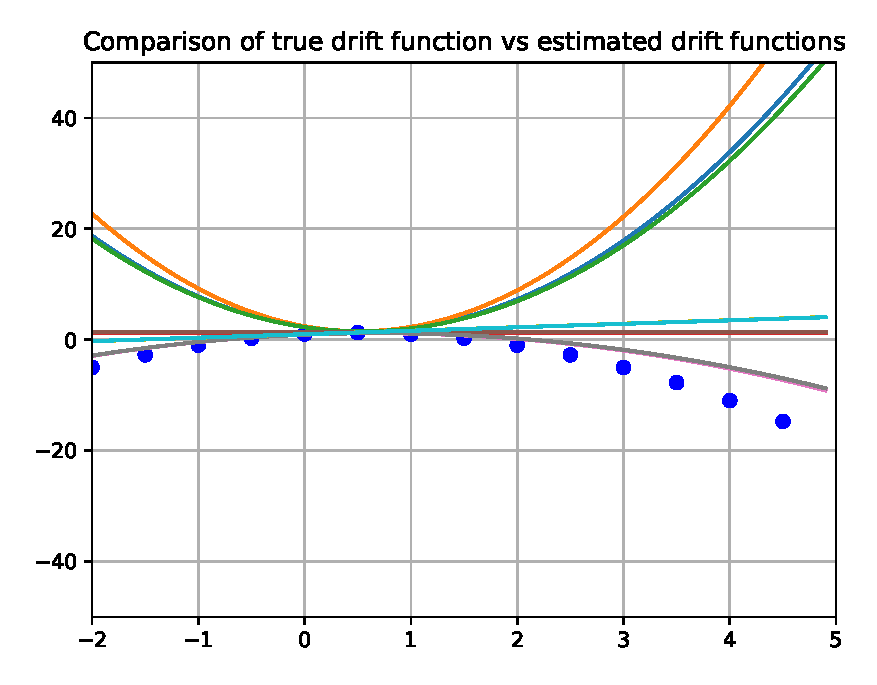
\includegraphics[height=1in]{../1dcode/varying_num_timeseries/plots/drift_comparison.eps}
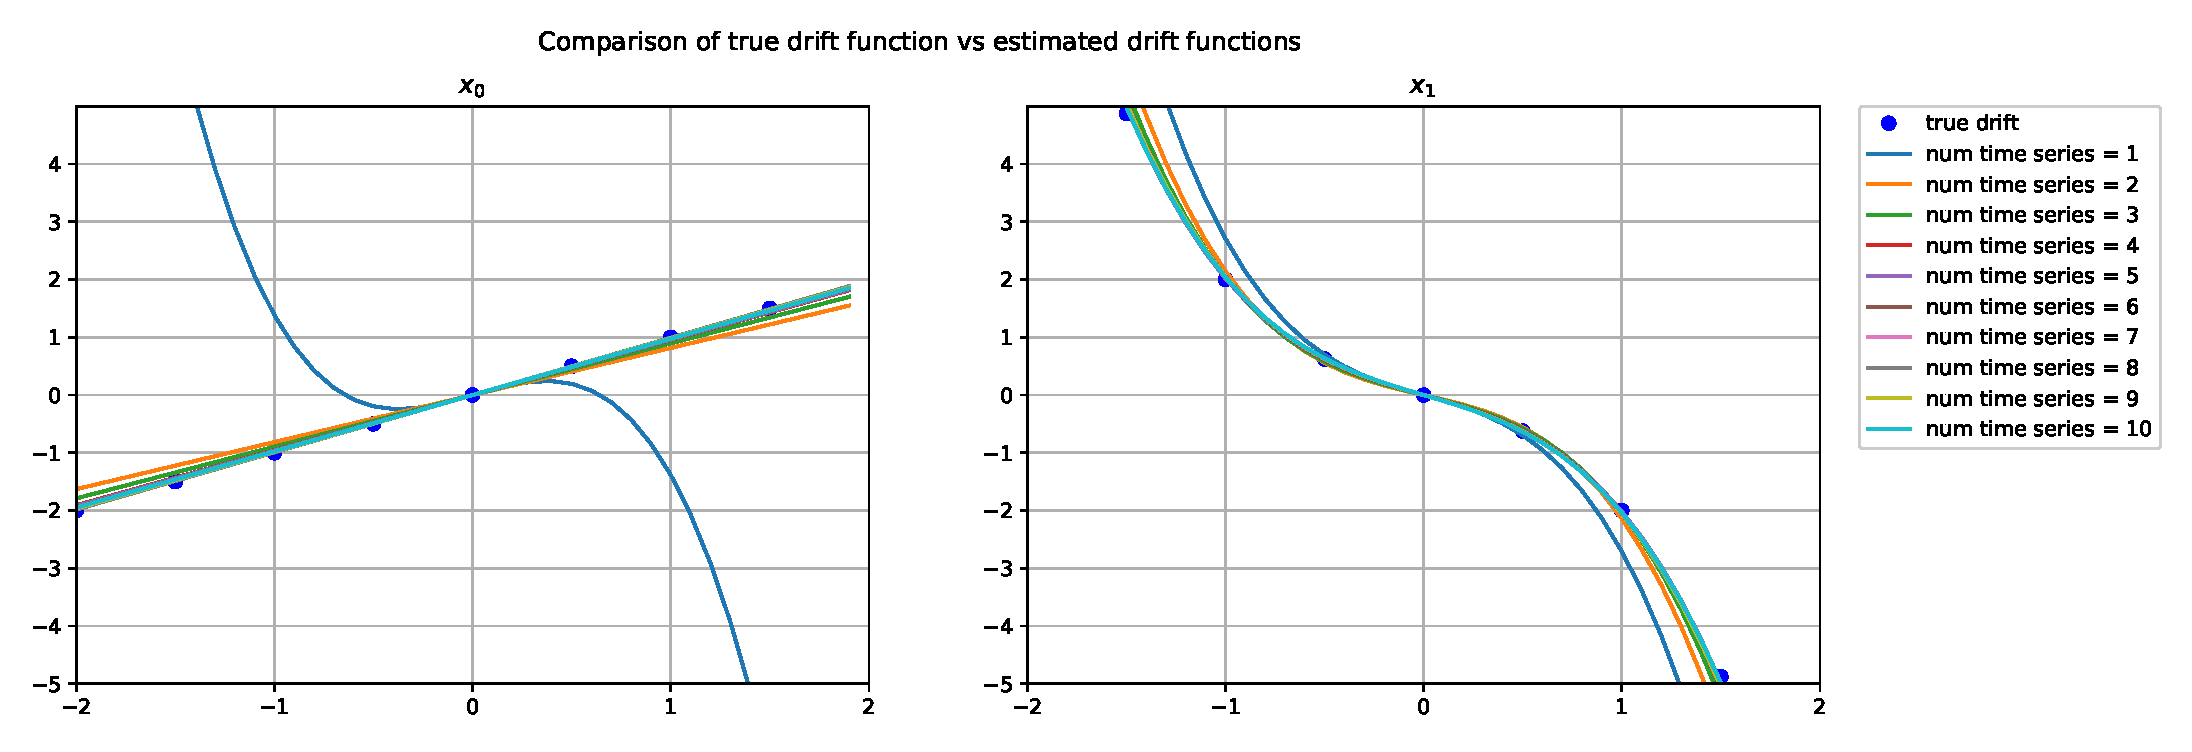
\includegraphics[height=1in]{../2dcode/varying_num_timeseries/plots/drift_comparison.eps}
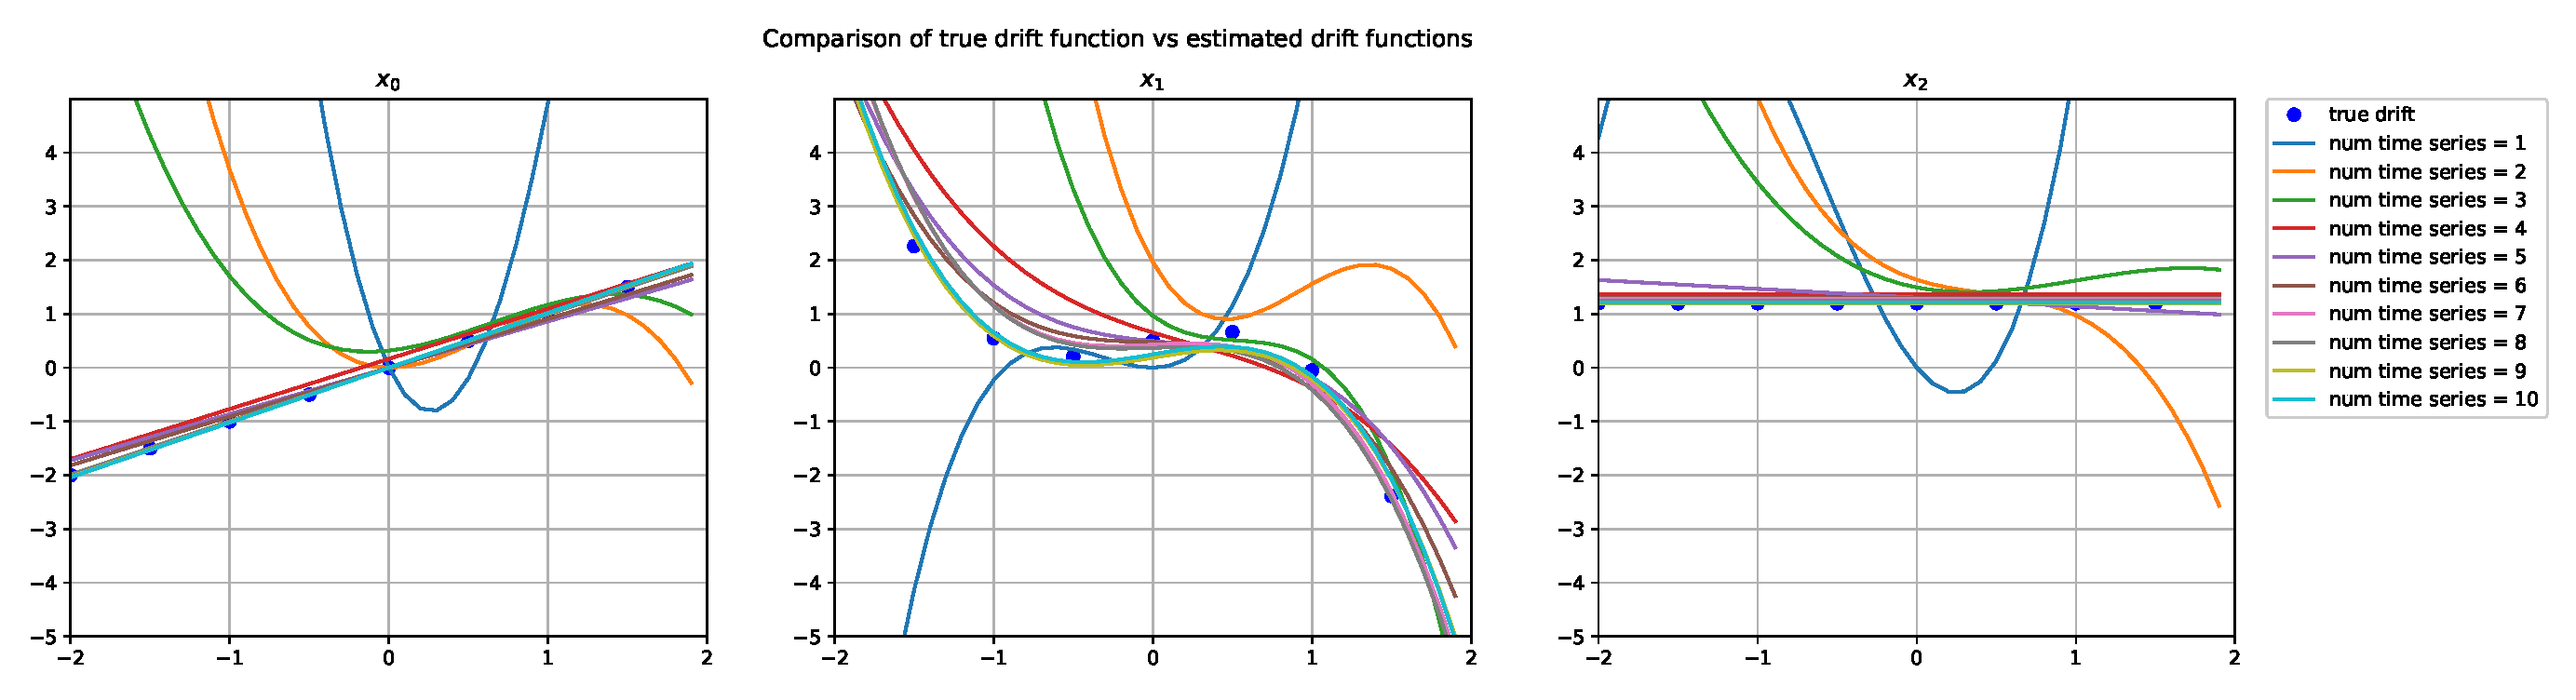
\includegraphics[height=1in]{../3ddampedduffing/varying_num_timeseries/plots/drift_comparison.eps}
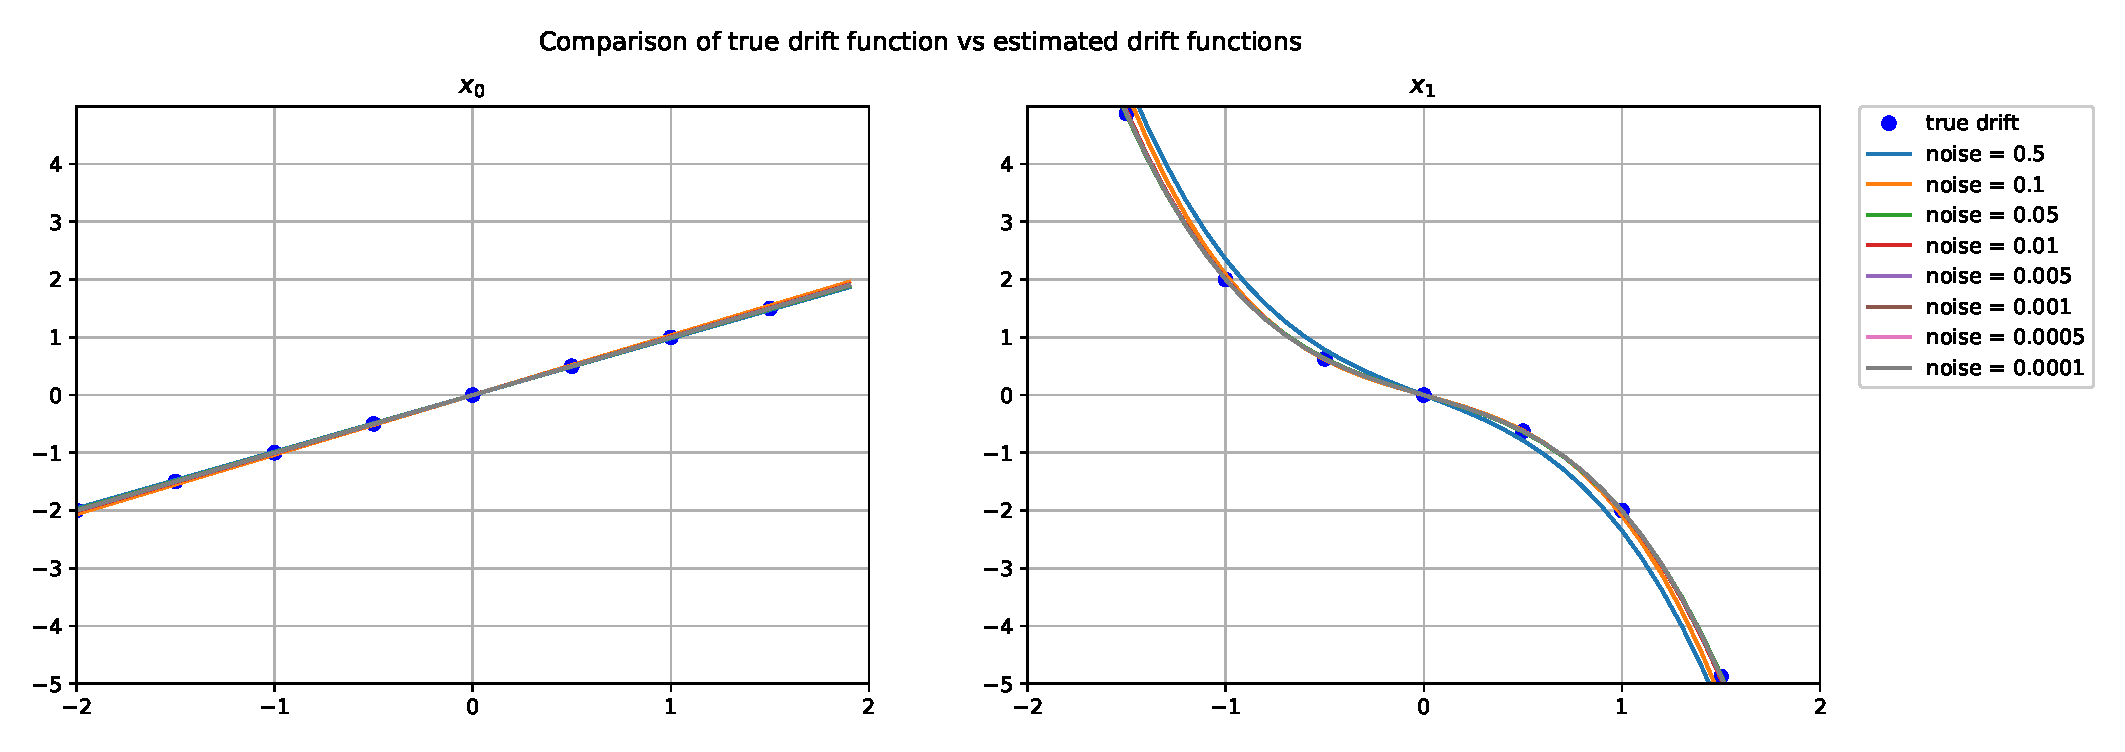
\includegraphics[height=1in]{../3dlorenz/varying_num_timeseries/plots/drift_comparison.eps}
\caption{Varying number of time series.}
\label{fig:exp1}
\end{figure}

\paragraph{Experiment 2: Varying Length of Time Series.} Here we vary data volume by stepping the length $L+1$ of the time series from $L+1 = 11$ to $L+1 = 101$, keeping the number of time series fixed at $S=10$.

\begin{figure}[th]
\includegraphics[height=1in]{../1dcode/random_timepoints/plots/hermite.eps}
\includegraphics[height=1in]{../2dcode/random_timepoints/plots/hermite.eps}
\includegraphics[height=1in]{../3ddampedduffing/random_timepoints/plots/hermite.eps}
\includegraphics[height=1in]{../3dlorenz/random_timepoints/plots/hermite.eps}
\caption{Varying length of time series.}
\label{fig:exp2}
\end{figure}

\paragraph{Experiment 3: Varying Noise Strength.} Here we vary the noise strength $\gamma$, stepping from $0.5$ to $0.0001$ while keeping other parameters constant.  Specifically, we take $S=10$ time series each of length $L+1 = 101$.
\begin{figure}[th]
\includegraphics[height=1in]{../1dcode/varying_noise/plots/hermite.eps}
\includegraphics[height=1in]{../2dcode/varying_noise/plots/hermite.eps}
\includegraphics[height=1in]{../3ddampedduffing/varying_noise/plots/hermite.eps}
\includegraphics[height=1in]{../3dlorenz/varying_noise/plots/hermite.eps}
\caption{Varying noise strength.}
\label{fig:exp2}
\end{figure}

\paragraph{Experiment 4: Varying Data Augmentation.} 
Here we vary the number $F$ of interleaved diffusion bridge samples from $F=1$ to $F=9$.  Note that for $F=1$, no diffusion bridge is created; the likelihood is computed by applying the Gaussian transition density directly to the observed data.
\begin{figure}[th]
\includegraphics[height=1in]{../1dcode/varying_subintervals/plots/tp_51/hermite.eps}
\includegraphics[height=1in]{../2dcode/varying_subintervals/plots/tp_51/hermite.eps}
\includegraphics[height=1in]{../3ddampedduffing/varying_subintervals/plots/tp_51/hermite.eps}
\includegraphics[height=1in]{../3dlorenz/varying_subintervals/plots/tp_51/hermite.eps}
\caption{Varying length of the diffusion bridge.}
\label{fig:exp2}
\end{figure}

{\small
\bibliographystyle{abbrvnat}
\bibliography{results}
}

\end{document}
